

    \item A uniform circular disc of mass 1.5 kg and radius 0.5 m is initially at rest on a horizontal frictionless surface. Three forces of equal magnitude $F = 0.5$ N are applied simultaneously along the three sides of an equilateral triangle XYZ with its vertices on the perimeter of the disc (see figure). One second after applying the forces, the angular speed of the disc in $\text{rad s}^{-1}$ is \underline{\hspace{2.5 cm}}
        \begin{center}
            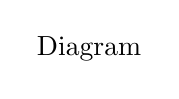
\begin{tikzpicture}
                \node {Diagram};
            \end{tikzpicture}
        \end{center}

